\chapter{Semileptonic DNN Data sideband and MC Signal Region Checks}
\label{sec:SL_DNN_Sideband_Check}

To ensure the diphoton mass is not shaped by the semileptonic multiclass DNN, the sidebands of the diphoton mass distribution are shown for different selections 
made on the DNN output score, shown in the figures below. No evident shaping is seen, and therefore no bias is expected from the DNN. 

\begin{figure}[H]
    \setcounter{subfigure}{0}
    \centering
    \subfloat[DNN score $>$ 0.0]{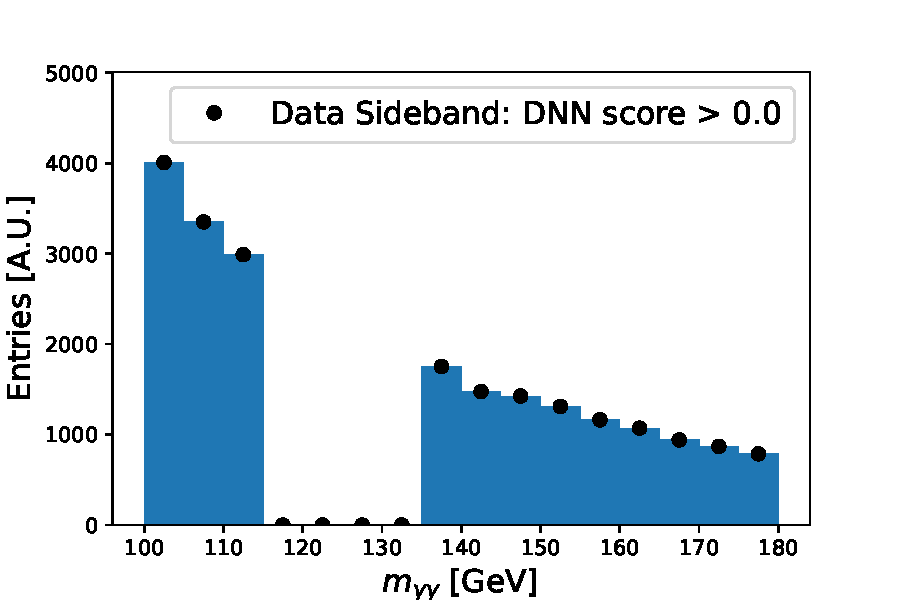
\includegraphics[width=0.45\textwidth]{Sections/HHWWgg/images/SL_DNN_Sideband_and_MCSR_Check/Data_Sideband_DNNgt_0p0.pdf}}
    \qquad
    \subfloat[DNN score $>$ 0.5]{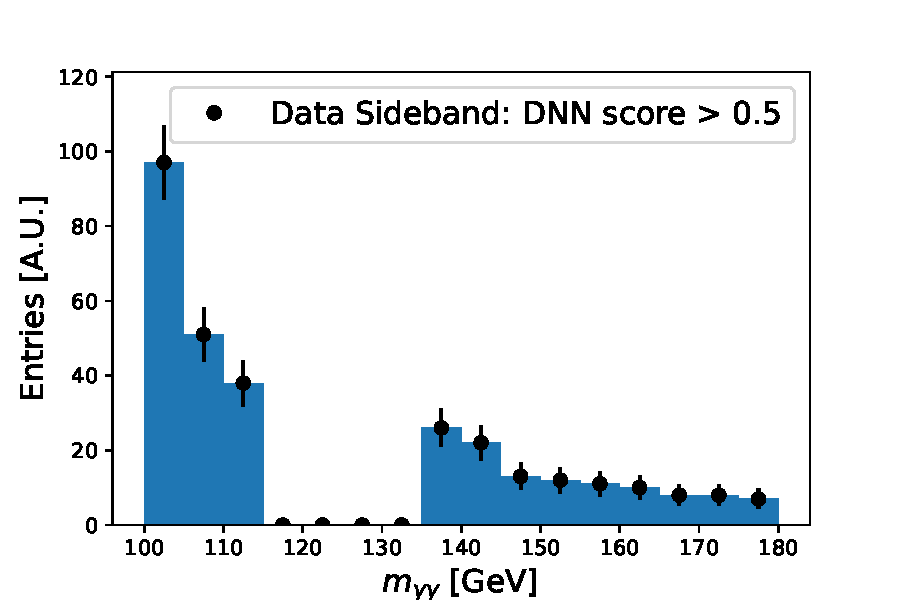
\includegraphics[width=0.45\textwidth]{Sections/HHWWgg/images/SL_DNN_Sideband_and_MCSR_Check/Data_Sideband_DNNgt_0p5.pdf}}
    \caption{Di-photon mass data sideband: Taken from Run 2 data.}
\end{figure}

\begin{figure}[H]
    \setcounter{subfigure}{0}
    \centering
    \subfloat[DNN score $>$ 0.65]{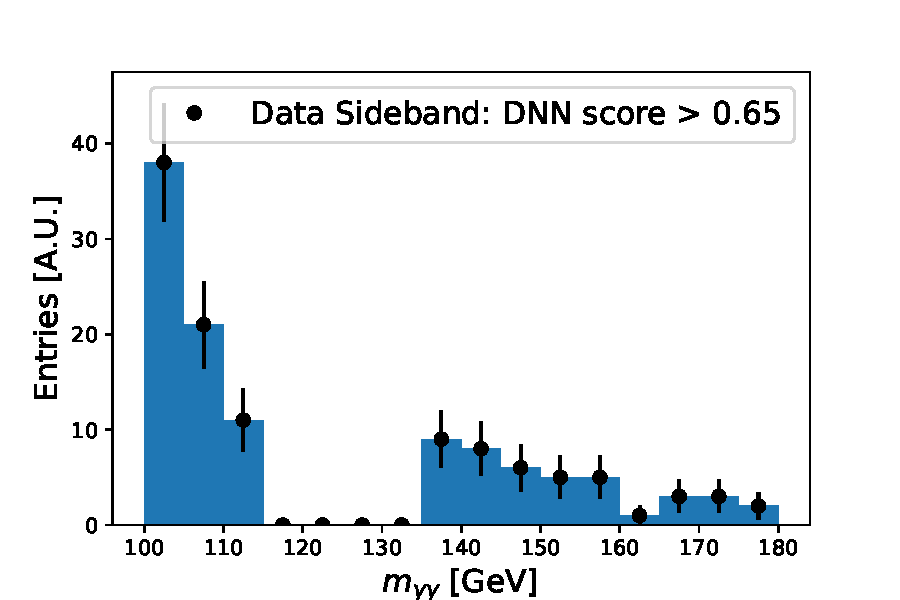
\includegraphics[width=0.45\textwidth]{Sections/HHWWgg/images/SL_DNN_Sideband_and_MCSR_Check/Data_Sideband_DNNgt_0p65.pdf}}
    \qquad
    \subfloat[DNN score $>$ 0.7]{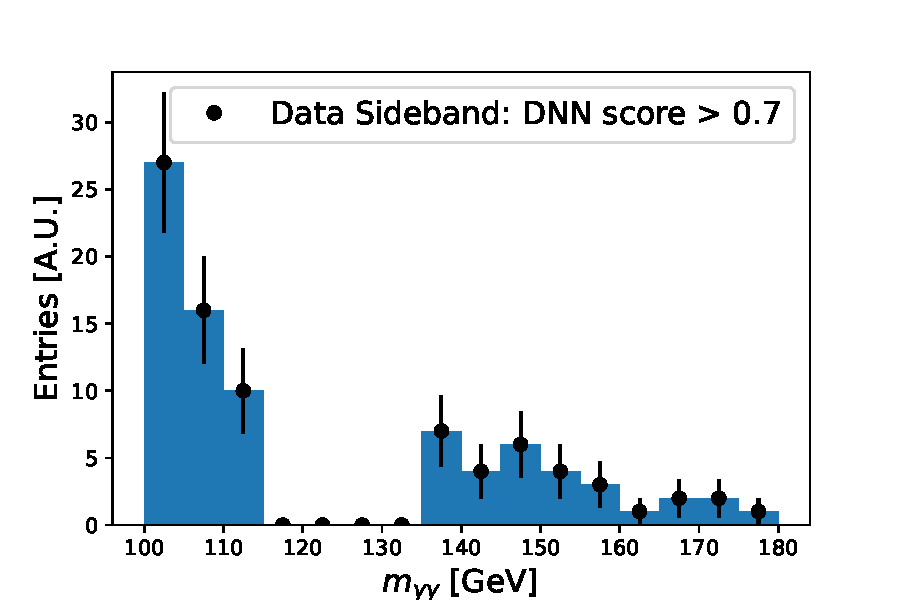
\includegraphics[width=0.45\textwidth]{Sections/HHWWgg/images/SL_DNN_Sideband_and_MCSR_Check/Data_Sideband_DNNgt_0p7.pdf}}
    \caption{Di-photon mass data sideband: Taken from Run 2 data.}
\end{figure}

\newpage 

\begin{figure}[H]
    \setcounter{subfigure}{0}
    \centering
    \subfloat[DNN score $>$ 0.75]{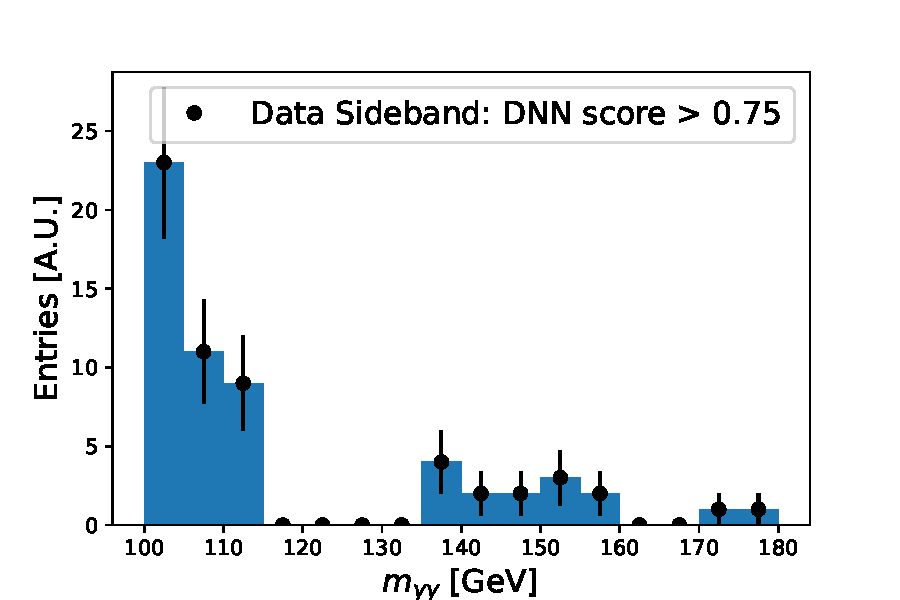
\includegraphics[width=0.45\textwidth]{Sections/HHWWgg/images/SL_DNN_Sideband_and_MCSR_Check/Data_Sideband_DNNgt_0p75.pdf}}
    \qquad
    \subfloat[DNN score $>$ 0.8]{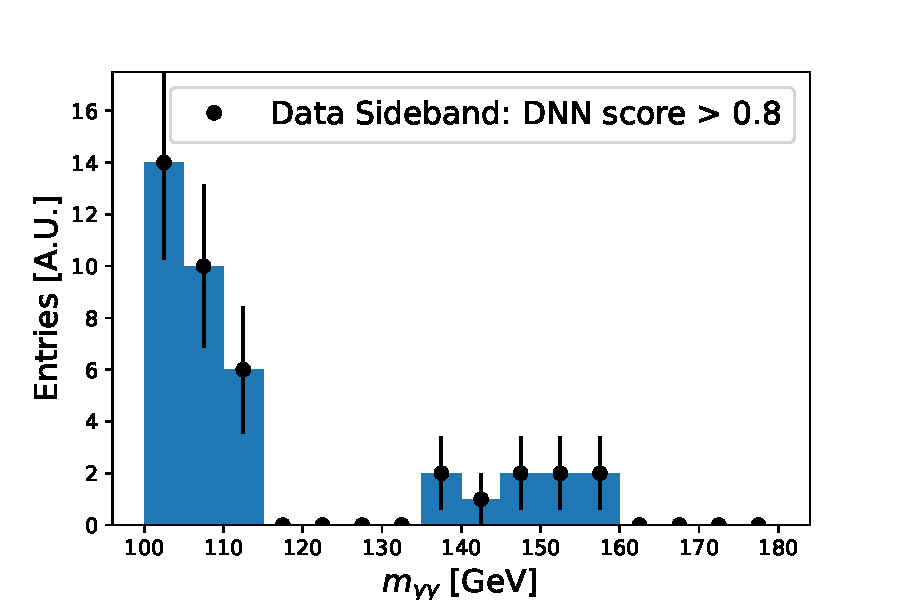
\includegraphics[width=0.45\textwidth]{Sections/HHWWgg/images/SL_DNN_Sideband_and_MCSR_Check/Data_Sideband_DNNgt_0p8.pdf}}
    \caption{Di-photon mass data sideband: Taken from Run 2 data.}
\end{figure}

\begin{figure}[H]
    \setcounter{subfigure}{0}
    \centering
    \subfloat[DNN score $>$ 0.85]{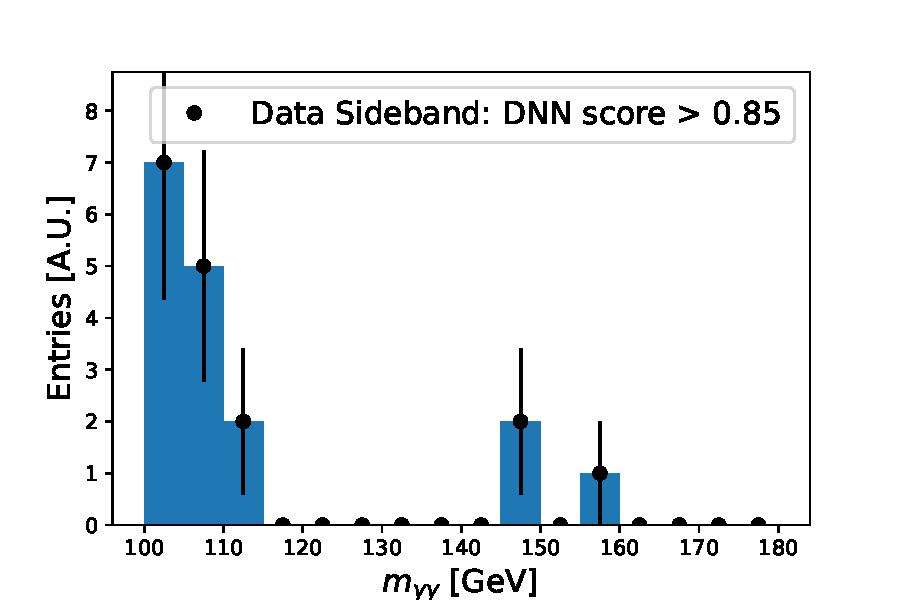
\includegraphics[width=0.45\textwidth]{Sections/HHWWgg/images/SL_DNN_Sideband_and_MCSR_Check/Data_Sideband_DNNgt_0p85.pdf}}
    \qquad
    \subfloat[DNN score $>$ 0.9]{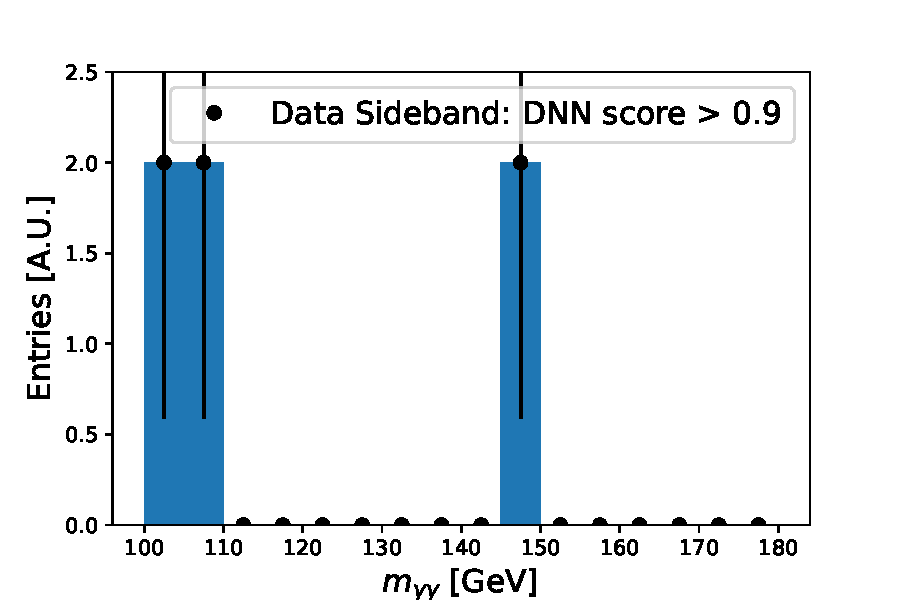
\includegraphics[width=0.45\textwidth]{Sections/HHWWgg/images/SL_DNN_Sideband_and_MCSR_Check/Data_Sideband_DNNgt_0p9.pdf}}
    \caption{Di-photon mass data sideband: Taken from Run 2 data.}
\end{figure}

In addition, the diphoton mass of the background MC which the DNN trains on is plotted in the mass range 100 to 180 GeV, including the signal region, for different DNN selections, 
shown in the figured below. No evident shaping is seen within the statistical uncertainty of the check, and therefore no bias is expected from the DNN. 

\begin{figure}[H]
    \setcounter{subfigure}{0}
    \centering
    \subfloat[DNN score $>$ 0.0]{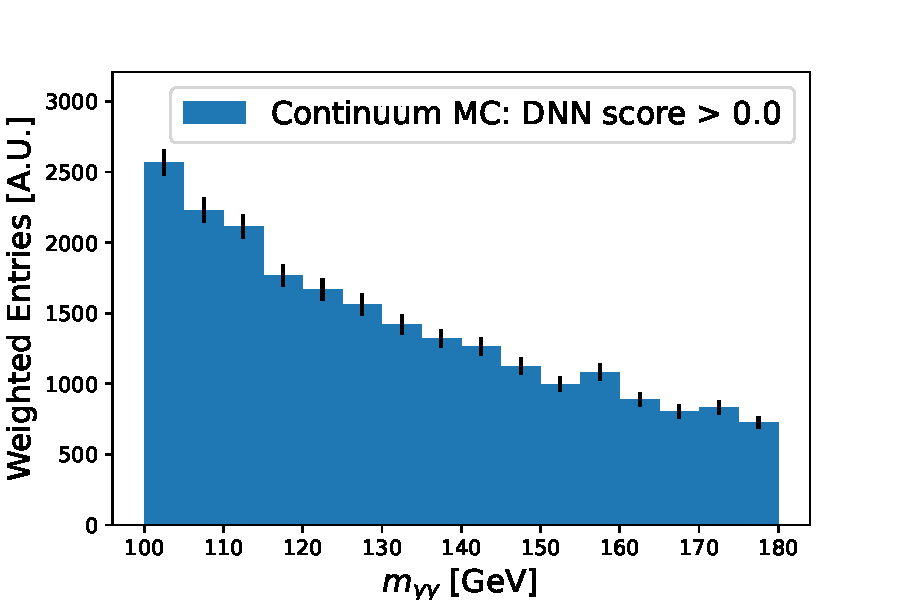
\includegraphics[width=0.45\textwidth]{Sections/HHWWgg/images/SL_DNN_Sideband_and_MCSR_Check/Continuum_MC_DNNgt_0p0.pdf}}
    \qquad
    \subfloat[DNN score $>$ 0.5]{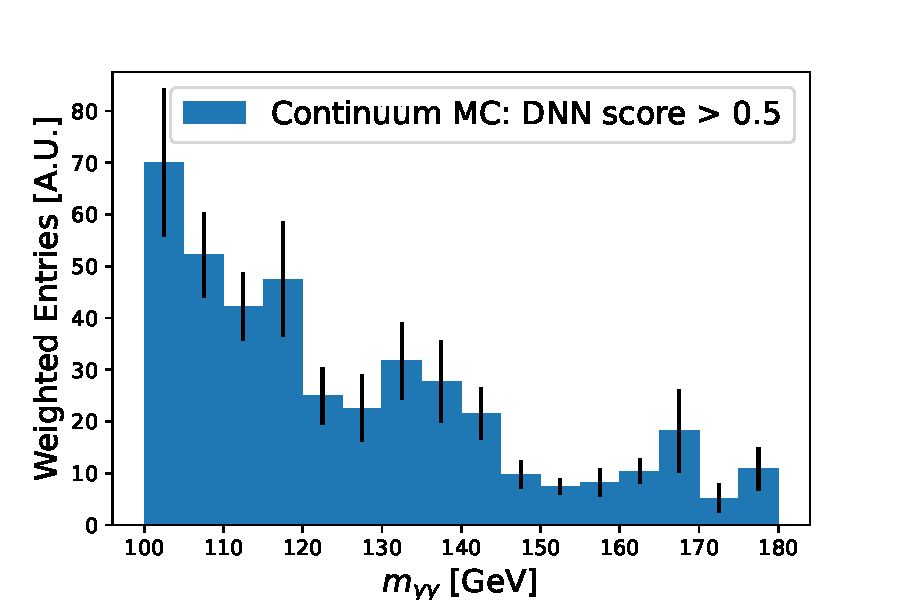
\includegraphics[width=0.45\textwidth]{Sections/HHWWgg/images/SL_DNN_Sideband_and_MCSR_Check/Continuum_MC_DNNgt_0p5.pdf}}
    \caption{Di-photon mass of MC in the data sideband and signal region: Taken from MC used for DNN training.}
\end{figure}

\begin{figure}[H]
    \setcounter{subfigure}{0}
    \centering
    \subfloat[DNN score $>$ 0.65]{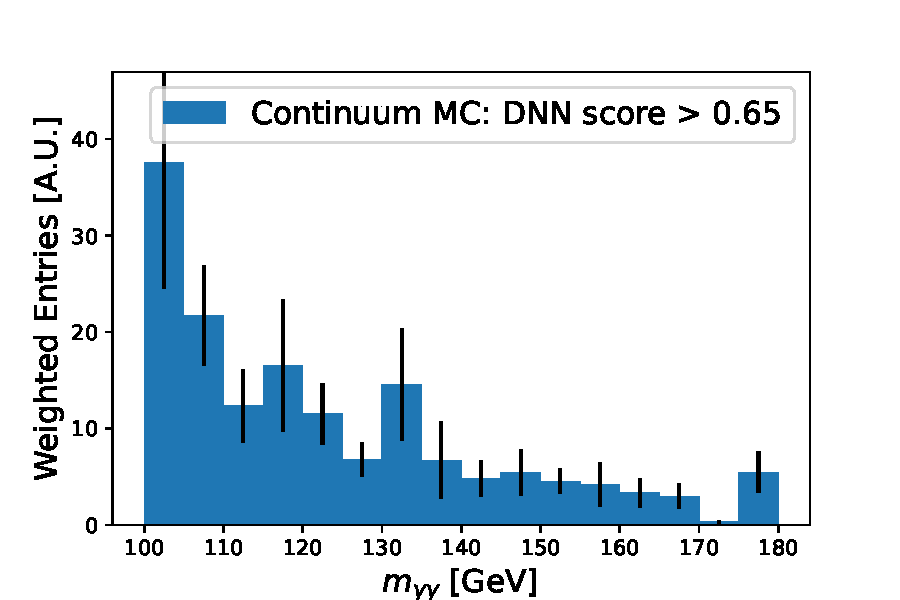
\includegraphics[width=0.45\textwidth]{Sections/HHWWgg/images/SL_DNN_Sideband_and_MCSR_Check/Continuum_MC_DNNgt_0p65.pdf}}
    \qquad
    \subfloat[DNN score $>$ 0.7]{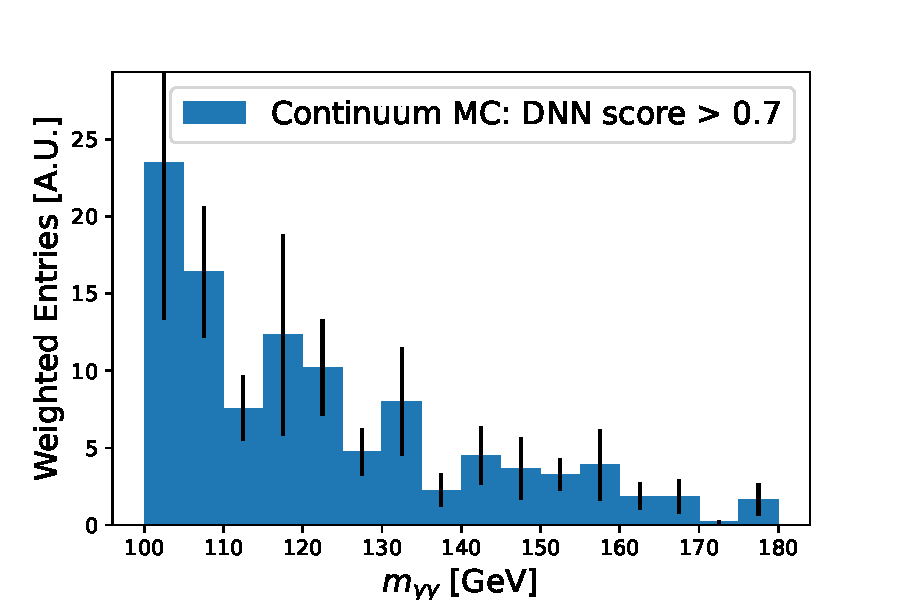
\includegraphics[width=0.45\textwidth]{Sections/HHWWgg/images/SL_DNN_Sideband_and_MCSR_Check/Continuum_MC_DNNgt_0p7.pdf}}
    \caption{Di-photon mass of MC in the data sideband and signal region: Taken from MC used for DNN training.}
\end{figure}

\newpage 

\begin{figure}[H]
    \setcounter{subfigure}{0}
    \centering
    \subfloat[DNN score $>$ 0.75]{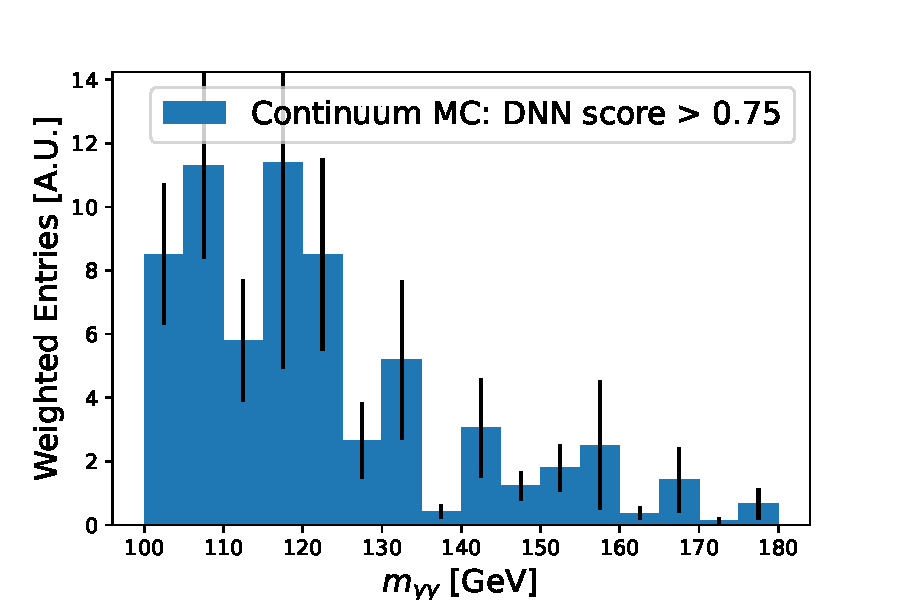
\includegraphics[width=0.45\textwidth]{Sections/HHWWgg/images/SL_DNN_Sideband_and_MCSR_Check/Continuum_MC_DNNgt_0p75.pdf}}
    \qquad
    \subfloat[DNN score $>$ 0.8]{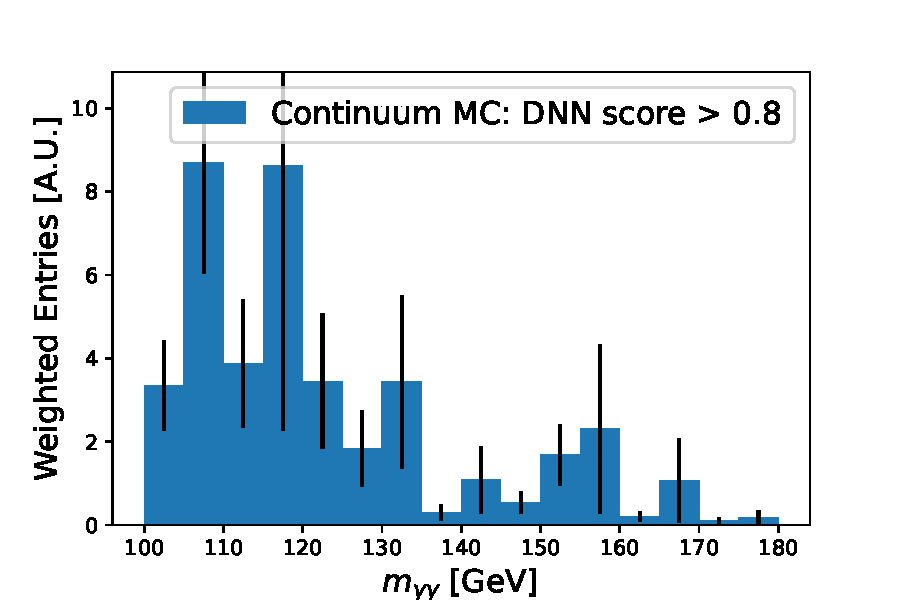
\includegraphics[width=0.45\textwidth]{Sections/HHWWgg/images/SL_DNN_Sideband_and_MCSR_Check/Continuum_MC_DNNgt_0p8.pdf}}
    \caption{Di-photon mass of MC in the data sideband and signal region: Taken from MC used for DNN training.}
\end{figure}

\begin{figure}[H]
    \setcounter{subfigure}{0}
    \centering
    \subfloat[DNN score $>$ 0.85]{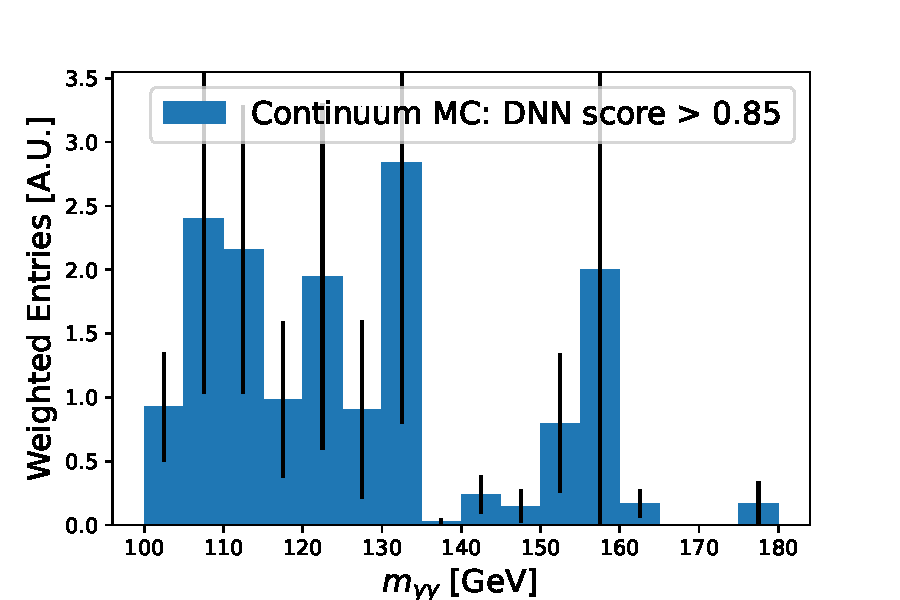
\includegraphics[width=0.45\textwidth]{Sections/HHWWgg/images/SL_DNN_Sideband_and_MCSR_Check/Continuum_MC_DNNgt_0p85.pdf}}
    \qquad
    \subfloat[DNN score $>$ 0.9]{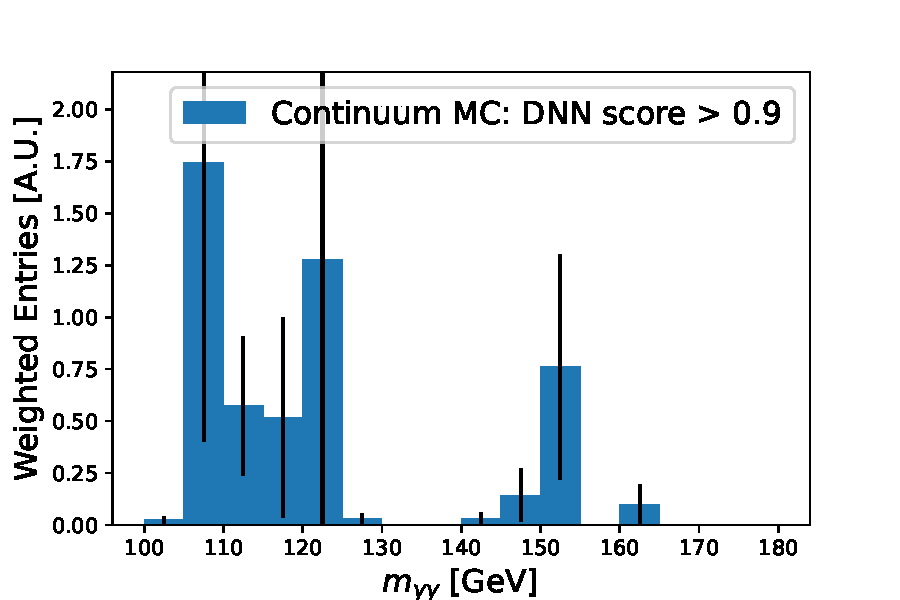
\includegraphics[width=0.45\textwidth]{Sections/HHWWgg/images/SL_DNN_Sideband_and_MCSR_Check/Continuum_MC_DNNgt_0p9.pdf}}
    \caption{Di-photon mass of MC in the data sideband and signal region: Taken from MC used for DNN training.}
\end{figure}